\documentclass{beamer}
\usepackage[utf8]{inputenc}
\usepackage[T1]{fontenc}
% \usepackage{amscd, amsfonts, amsmath, amssymb, amstext, amsthm, caption, epsfig, fancyhdr, float, graphicx, latexsym, mathtools, multicol, multirow, algorithm, chngcntr}
\usepackage[english, french]{babel}
\usepackage{booktabs}

\usepackage{amsmath,amssymb}
\usepackage{graphicx}
\usepackage{caption}
\usepackage{subfig}
\usepackage{xspace}
\usepackage{fourier}

\usepackage{tikz}
\usetikzlibrary{shapes,arrows}
\usepackage{tkz-graph}
\usetikzlibrary{automata,arrows,positioning,calc}
\usetikzlibrary{positioning}
\usetikzlibrary{fit}
\usetikzlibrary{backgrounds}
\usetikzlibrary{calc}
\usetikzlibrary{shapes}
\usetikzlibrary{mindmap}
\usetikzlibrary{decorations.text}

% \theoremstyle{definition} % insert bellow all blocks you want in normal text
% \newtheorem{definition}{Definition}



% tikzmark command, for shading over items
\newcommand{\tikzmark}[1]{\tikz[overlay,remember picture] \node (#1) {};}
% Define block styles
\tikzstyle{decision} = [diamond, draw, fill=blue!20,
    text width=4.5em, text badly centered, node distance=3cm, inner sep=0pt]
\tikzstyle{block} = [rectangle, draw, fill=blue!20,
    text width=5em, text centered, rounded corners]
\tikzstyle{line} = [draw]
\tikzstyle{cloud} = [draw, ellipse,fill=red!20, node distance=3cm,
    minimum height=2em]

\usepackage[most]{tcolorbox}

\setbeamertemplate{blocks}[rounded][shadow=true] % use rounded blocks with standard beamer shadow

\newcommand*{\warning}{\fontencoding{U}\fontfamily{futs}\selectfont\char 66\relax}

% Distributions.
\newcommand*{\UnifDist}{\mathsf{Unif}}
\newcommand*{\ExpDist}{\mathsf{Exp}}
\newcommand*{\DepExpDist}{\mathsf{DepExp}}
\newcommand*{\GammaDist}{\mathsf{Gamma}}
\newcommand*{\LognormalDist}{\mathsf{LogNorm}}
\newcommand*{\WeibullDist}{\mathsf{Weib}}
\newcommand*{\ParetoDist}{\mathsf{Par}}
\newcommand*{\NormalDist}{\mathsf{Norm}}

\newcommand*{\GeometricDist}{\mathsf{Geom}}
\newcommand*{\NegBinomialDist}{\mathsf{NegBin}}
\newcommand*{\PoissonDist}{\mathsf{Poisson}}
\newcommand*{\BivariatePoissonDist}{\mathsf{BPoisson}}
\newcommand*{\CyclicalPoissonDist}{\mathsf{CPoisson}}

\newcommand*{\iid}{\textbf{iid}\@\xspace}
\newcommand*{\pdf}{\textbf{pdf}\@\xspace}
\newcommand*{\cdf}{\textbf{cdf}\@\xspace}
\newcommand*{\pmf}{\textbf{pmf}\@\xspace}
\newcommand*{\abc}{{\textbf{abc}}\@\xspace}
\newcommand*{\smc}{\textbf{smc}\@\xspace}
\newcommand*{\mcmc}{\textbf{mcmc}\@\xspace}
\newcommand*{\ess}{\textbf{ess}\@\xspace}
\newcommand*{\mle}{\textbf{mle}\@\xspace}
\newcommand*{\bic}{\textbf{bic}\@\xspace}
\newcommand*{\kde}{\textbf{kde}\@\xspace}
\newcommand*{\glm}{\textbf{glm}\@\xspace}
\newcommand*{\xol}{\textbf{xol}\@\xspace}
\newcommand*{\cpu}{\textbf{cpu}\@\xspace}
\newcommand*{\gpu}{\textbf{gpu}\@\xspace}
\newcommand*{\arm}{\textbf{arm}\@\xspace}

\def \si {\sigma}
\def \la {\lambda}
\def \al {\alpha}
% \def\e*{\end{eqnarray*}}
\def \di{\displaystyle}

\def \E{\mathbb E}
\def \N{\mathbb N}
\def \Z{\mathbb Z}
\def \NZ{\mathbb{N}_0}
\def \I{\mathbb I}
\def \w{\widehat}
\def \P {\mathbb P}
\def \V{\mathbb V}


\newcommand{\CL}{\mathbb{C}}
\newcommand{\RL}{\mathbb{R}}
\newcommand{\nat}{{\mathbb N}}
\newcommand{\Laplace}{\mathscr{L}}
\newcommand{\e}{\mathrm{e}}
\newcommand{\ve}{\bm{\mathrm{e}}} % vector e

\renewcommand{\L}{\mathcal{L}} % e.g. L^2 loss.

\newcommand{\ih}{\mathrm{i}}
\newcommand{\oh}{{\mathrm{o}}}
\newcommand{\Oh}{{\mathcal{O}}}
\newcommand{\Exp}{\mathbb{E}}

\newcommand{\Norm}{\mathcal{N}}
\newcommand{\LN}{\mathcal{LN}}
\newcommand{\SLN}{\mathcal{SLN}}

\renewcommand{\Pr}{\mathbb{P}}
\newcommand{\Ind}{\mathbb I}
\newcommand\bfsigma{\bm{\sigma}}
\newcommand\bfSigma{\bm{\Sigma}}
\newcommand\bfLambda{\bm{\Lambda}}
\newcommand{\stimes}{{\times}}
\def \limsup{\underset{n\rightarrow+\infty}{\overline{\lim}}}
\def \liminf{\underset{n\rightarrow+\infty}{\underline{\lim}}}




% vertical separator macro
\newcommand{\vsep}{
  \column{0.0\textwidth}
    \begin{tikzpicture}
      \draw[very thick,black!10] (0,0) -- (0,7.3);
    \end{tikzpicture}
}
\newcommand\blfootnote[1]{%
  \begingroup
  \renewcommand\thefootnote{}\footnote{#1}%
  \addtocounter{footnote}{-1}%
  \endgroup
}

% More space between lines in align
% \setlength{\mathindent}{0pt}

% Beamer theme
\usetheme{ZMBZFMK}
\usefonttheme[onlysmall]{structurebold}
\mode<presentation>
\setbeamercovered{transparent=10}

% align spacing
\setlength{\jot}{0pt}

\setbeamertemplate{navigation symbols}{}%remove navigation symbols

\title[BLOCKASTICS II]{Stochastic Models for blockchain analysis}
\subtitle{Simple models for blockchain performance analysis}
\author{Pierre-O. Goffard}
\institute[ISFA]{Institut de Science Financières et d'Assurances\\
 \texttt{pierre-olivier.goffard@univ-lyon1.fr}}
\date{\today}
\titlegraphic{\includegraphics[width=2.5cm]{../../Figures/bfs_logo.png}} 

\begin{document}
\begin{frame}
  \titlepage
\end{frame}
\begin{frame}{The three dimensions of blockchain analysis}
\tableofcontents
% \begin{enumerate}
%   \item Security of PoW blockchain
%   \item Decentralization in PoS blockchain
%   \item Blockhain efficiency
% \end{enumerate}
\end{frame}
\section{Security of PoW blockchain}
\begin{frame}{Double spending attack}
\scriptsize
\begin{enumerate}
\item Mary transfers 10 BTCs to John
\item The transaction is recorded in the public branch of the blockchain and John ships the good.
\item Mary transfers to herself the exact same BTCs
\item The malicious transaction is recorded into a private branch of the blockchain
\begin{itemize}
  \scriptsize
\item Mary has friends among the miners to help her out
\item The two chains are copycat up to the one transaction
\end{itemize}
\end{enumerate}
\begin{tcolorbox}[enhanced,drop shadow, title=Fact (Bitcoin has only one rule)]
The longest chain is to be trusted
\end{tcolorbox}
\end{frame}
\begin{frame}{Double spending in practice}
\scriptsize
Vendor are advised to wait for $\alpha\in\mathbb{N}$ of confirmations so that the honest chain is ahead of the dishonest one.
\begin{center}
\begin{tikzpicture}[-, >=stealth', auto, semithick, node distance=1cm]
% \tikzstyle{block} = [rectangle, draw, fill=blue!20,
%     text width=5em, text centered, rounded corners]
\tikzstyle{block}=[rectangle, fill=black,draw=black,thick,text=black,scale=0.6]
\tikzstyle{block}=[rectangle, fill=white,draw=black,thick,text=black,scale=0.8]
\tikzstyle{confirmed block}=[rectangle, fill=white,draw=blue,thick,text=black,scale=0.8]
\tikzstyle{bad block}=[rectangle, fill=white,draw=red,thick,text=black,scale=0.8]
\node[block]    (1)                     {\tiny $\text{M}\rightarrow \text{J}$};
\node[block]    (2)[right of=1]                     {};
\node[block]    (3)[right of=2]                     {};
\node[block]    (4)[right of=3]                     {};
\node[confirmed block]    (5)[right of=4]                     {};

\node[bad block]    (6)[below of=1]         {\tiny $\text{M}\rightarrow \text{M}$};
\node[block]    (7)[right of=6]         {};
\node[block]    (8)[right of=7]         {};
\path
(1) edge[ left]     node{}     (2)
(2) edge[ left]     node{}     (3)
(3) edge[ left]     node{}     (4)
(4) edge[ left]     node{}     (5)
(6) edge[ left]     node{}     (7)
(7) edge[ left]     node{}     (8);

\end{tikzpicture}
\end{center}
In the example, vendor awaits $\alpha = 4$ confirmations, the honest chain is ahead of the dishonest one by $z = 2$ blocks.
\begin{tcolorbox}[enhanced,drop shadow, title=Fact (PoW is resistant to double spending)]
\begin{itemize}
\item Attacker does not own the majority of computing power 
\item Suitable $\alpha$ 
\end{itemize}
Double spending is unlikely to succeed.
\end{tcolorbox}
\tiny
\begin{thebibliography}{1}
\bibitem{Na08}
S.~Nakamoto, ``Bitcoin: A peer-to-peer electronic cash system.'' Available at
  \href{https://bitcoin.org/bitcoin.pdf}{https://bitcoin.org/bitcoin.pdf},
  2008.
  
\end{thebibliography}

\end{frame}
\begin{frame}{Mathematical set up}
\scriptsize
Assume that
\begin{itemize}
\item $R_0=z\geq1$ (the honest chain is z blocks ahead)
\item at each time unit a block is created
\begin{itemize}
  \scriptsize
\item[$\hookrightarrow$] in the honest chain with probability $p$
\item[$\hookrightarrow$] in the dishonest chain with probability $q=1-p$
\end{itemize}
\end{itemize}
The process $(R_n)_{n\geq0}$ is a random walk on $\mathbb{Z}$ with
$$R_n=z+Y_1+\ldots+Y_n,$$
where $Y_1,\ldots,Y_n$ are the \textbf{i.i.d.} steps of the random walk. 

\end{frame}
\begin{frame}{Double spending rate of success}
\scriptsize
Double spending occurs at time
$$
\tau_z=\inf\{n\in \mathbb{N}\text{ ; }R_n=0\}.
$$
\begin{tikzpicture}
  %Origin and axis
  \coordinate (O) at (0,0);
  \draw[->] (-1,0) -- (9,0) coordinate[label = {below:$n$}] (xmax);
  \draw[->] (0,-0.5) -- (0,3) coordinate[label = {left:$Z_n$}] (ymax);
  %Lower linear boundary

 
  %Stochastic process trajectory
  
  \draw (0,0) node[tublue,left] {} node{};
  \draw[very thick,tublue,-] (0,1) -- (1,1) node[pos=0.5, above] {} ;
  \draw[very thick,dashed,tublue] (1,1) -- (1,1.5) node[pos=0.5, right] {};
  \draw[very thick,tublue,-] (1,1.5) -- (2,1.5) node[pos=0.5, above] {};
  \draw[very thick,dashed,tublue] (2,1.5) -- (2,2) node[pos=0.5, right] {};
  \draw[very thick,tublue,-] (2,2) -- (3,2) node[pos=0.5, above] {};
  \draw[very thick,dashed,tublue] (3,2) -- (3,1.5) node[pos=0.5, right] {};
  \draw[very thick,tublue,-] (3,1.5) -- (4,1.5)node[pos=0.5, above] {};
  \draw[very thick,dashed,tublue] (4,1.5) -- (4,1) node[pos=0.5, right] {};  
  \draw[very thick,tublue,-] (4,1) -- (5,1) node[pos=0.5, above] {};
  \draw[very thick,dashed,tublue] (5,1) -- (5,0.5) node[pos=0.5, right] {};  
  \draw[very thick,tublue,-] (5,0.5) -- (6,0.5) node[pos=0.5, above] {};
  \draw[very thick,dashed,tublue,-] (6,0.5) -- (6,1) node[pos=0.5, above] {};
   \draw[very thick,tublue,-] (6,1) -- (7,1) node[pos=0.5, above] {};
    \draw[very thick,dashed,tublue,-] (7,1) -- (7,0.5) node[pos=0.5, above] {};
     \draw[very thick,tublue,-] (7,0.5) -- (8,0.5) node[pos=0.5, above] {};
     \draw[very thick,dashed,tublue,-] (8,0.5) -- (8,0) node[pos=0.5, above] {};
  %Jump Times
  \draw (1,0) node[black,below] {$1$} node{ \color{black}$\bullet$};
  \draw (2,0) node[black,below] {$2$} node{ \color{black}$\bullet$};
  \draw (3,0) node[black,below] {$3$} node{ \color{black}$\bullet$};
  \draw (4,0) node[black,below] {$4$} node{ \color{black}$\bullet$};
  \draw (5,0) node[black,below] {$5$} node{ \color{black}$\bullet$};
  \draw (6,0) node[black,below] {$6$} node{ \color{black}$\bullet$};
  \draw (7,0) node[black,below] {$7$} node{ \color{black}$\bullet$};
  \draw (8,0) node[black,below] {$8$} node{ \color{black}$\bullet$};
  %Level of the counting process
   \draw (0,0) node[black,below left] {$0$} node{ \color{black}$\bullet$};
   \draw (0,0.5) node[black,left] {$1$} node{ \color{black}$\bullet$};
   \draw (0,1) node[black,left] {$z=2$} node{ \color{black}$\bullet$};
   \draw (0,1.5) node[black,left] {$3$} node{ \color{black}$\bullet$};
   \draw (0,2) node[black,left] {$4$} node{ \color{black}$\bullet$};
   \draw (0,2.5) node[black,left] {$5$} node{ \color{black}$\bullet$};

  % %Aggregated Capital gains
%  \draw (0,1.5) node[blue,below right] {$\mu_1$} node{ \color{blue}$-$};
%  \draw (0,2.25) node[blue,left] {$\mu_2$} node{ \color{blue}$-$};
%  \draw (0,3.75) node[blue,left] {$\mu_3$} node{ \color{blue}$-$};
  %Ruin time = First-crossing time time
%  \draw (5,0) node[black,above right] {$\tau_u$} node{ \color{black}$\times$};
%  \draw[dotted,black] (0,3.28) -- (5,3.28);
%  \draw[dotted,black] (5,0) -- (5,3.28);
\end{tikzpicture}
\begin{tcolorbox}[enhanced,drop shadow, title=Double spending theorem]
If $p>q$ then the double-spending probability is given by
$$
\phi(z) = \mathbb{P}(\tau_z<\infty)=\left(\frac{q}{p}\right)^{z}.
$$
\end{tcolorbox}

\end{frame}

\begin{frame}[allowframebreaks]{Proof of the double spending theorem }
\scriptsize Analogy with the gambler's ruin problem. Using a first step analysis, we have 
\begin{equation}\label{eq:difference_equation}
\phi(z) = p\phi(z+1)+(1-p)\phi(z-1),\text{ }z\geq1.
\end{equation}
We also have the boundary conditions
\begin{equation}\label{eq:boundary_conditions_double_spending}
\phi(0) = 1\text{ and }\underset{z\rightarrow +\infty}{\lim}\phi(z) = 0
\end{equation}
Equation \eqref{eq:difference_equation} is a linear difference equation of order $2$ associated to the following characteristic equation
$$
px^2 - x + 1-p = 0
$$
which has two roots on the real line with 
$$
r_1 = 1, \text{ and }r_2 = \frac{1-p}{p}.
$$
The solution of \eqref{eq:difference_equation} is given by 
$$
\phi(z)=A+B\left(\frac{1-p}{p}\right)^z,
$$
where $A$ and $B$ are constant. Using the boudary conditions \eqref{eq:boundary_conditions_double_spending}, we deduce that
$$
\phi(z) = \left(\frac{1-p}{p}\right)^z
$$
as announced.
\end{frame}
\begin{frame}{Refinements of the double spending problem}
\scriptsize
The number of blocks $M$ found by the attacker until the honest miners find $\alpha$ blocks is a negative binomial random variable with \pmf
$$
\mathbb{P}(M = m) = \binom{\alpha+m-1}{m}p^\alpha q^m,\text{ }m\geq0.
$$
The number of block that the honest chain is ahead of the dishonest one is given by 
$$
Z= (\alpha-M)_+.
$$
Applying the law of total probability yields the probability of successful double spending with
$$
\mathbb{P}(\text{Double Spending}) = \mathbb{P}(M\geq \alpha) + \sum_{m = 0}^{\alpha - 1}\binom{\alpha+m-1}{m}q^{2\alpha} p^{2m}.
$$ 
\tiny


\begin{thebibliography}{1}
  \bibitem{rosenfeld2014analysis}
M.~Rosenfeld, ``Analysis of hashrate-based double spending,'' {\em arXiv
  preprint arXiv:1402.2009}, 2014.
  \bibitem{GRUNSPAN2018}
C.~Grunspan and R.~Perez-Marco, ``Double spend race,'' {\em
  International Journal of Theoretical and Applied Finance}, vol.~21,
  p.~1850053, dec 2018.
\end{thebibliography}

\end{frame}
\begin{frame}{Refinements of the double spending problem}
\scriptsize
Let the length of honest and dishonest chain be driven by counting processes
\begin{itemize}
\item Honest chain $\Rightarrow$ $z+N_t\text{ , }t\geq0$, where $z\geq1$.
\item Malicious chain $\Rightarrow$ $M_t\text{ , }t\geq0$
\item Study the distribution of the first-\textit{rendez-vous} time
$$
\tau_z=\inf\{t\geq0\text{ , } M_t=z+N_t\}.
$$
\end{itemize}
If $N_t\sim\text{Pois}(\lambda t)$ and $M_t\sim\text{Pois}(\mu t)$ such that $\lambda>\mu$ then 
$$
\phi(z) = \left(\frac{\mu}{\lambda}\right)^z,\text{ }z\geq 0.
$$
\tiny
\begin{thebibliography}{1}

\bibitem{Goffard2019}
P.-O. Goffard, ``Fraud risk assessment within blockchain transactions,'' {\em
  Advances in Applied Probability}, vol.~51, pp.~443--467, jun 2019.
\newblock \url{https://hal.archives-ouvertes.fr/hal-01716687v2}.

\bibitem{Bowden2020}
R.~Bowden, H.~P. Keeler, A.~E. Krzesinski, and P.~G. Taylor, ``Modeling and
  analysis of block arrival times in the bitcoin blockchain,'' {\em Stochastic
  Models}, vol.~36, pp.~602--637, jul 2020.
\end{thebibliography}

\end{frame}
\begin{frame}{Perspectives}
\begin{itemize}
\item Distribution of $\tau_z$? (To be discussed later)
\item Distribution of $Z$
\begin{itemize}
  \item[$\hookrightarrow$] Negative binomial when the length of the blockchain are driven by Poisson processes
  \item [$\hookrightarrow$] if not?
\end{itemize}
\end{itemize}
\end{frame}
\section{Decentralization in PoS blockchain}
\begin{frame}{Proof of Stake protocol}
\scriptsize
PoS is the most popular alternative to PoW.
\begin{itemize}
  \item A block validator is selected according to the number of native coins she owns
  \item Update the blockchain and receive a reward or do nothing  
\end{itemize}
Two problems 
\begin{itemize}
  \item[\warning] Nothing at stake $\Rightarrow$ Consensus postponed
  \item[\warning] Rich gets richer $\Rightarrow$ Risk of centralization
\end{itemize}

\end{frame}
\begin{frame}{Nothing-at-Stake}
\scriptsize
If given the opportunity a node will always append a new block
\begin{itemize}
  \item Everlasting fork if any
\end{itemize}
Perpetuating disagreement prevent users to exchange which lower the coin value.
\begin{tcolorbox}[enhanced,drop shadow, title=Theorem]
To get consensus faster and almost surely 
\begin{itemize}
  \item Set a minimum stake to outweight the benefit of the reward
  \item Set up a modest reward schedule $\sum_{t = 1}^\infty \text{r}_t<\infty$
\end{itemize}
\end{tcolorbox}
\tiny
\begin{thebibliography}{1}

\bibitem{Saleh2020}
F.~Saleh, ``Blockchain without waste: Proof-of-stake,'' {\em The Review of
  Financial Studies}, vol.~34, pp.~1156--1190, jul 2020.
\end{thebibliography}
\end{frame}
\begin{frame}{Risk of centralization ?}
\scriptsize
\begin{columns}
\begin{column}{0.5\textwidth}
Block appending process
\begin{itemize}
  \item Draw a coin at random
  \item The owner of the coin append a block and collect the reward
  \item The block appender is more likely to get selected during the next round
\end{itemize}
\end{column}
\begin{column}{0.5\textwidth}
Similar to Polya's urn 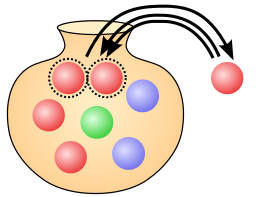
\includegraphics[scale=0.1]{../../Figures/poly_urn.png}
\begin{itemize}
  \item Consider an urn of $N$ balls of color in $E=\{1,\ldots, p\}$
  \item Draw a ball of color $x\in E$
  \item Replace the ball together with $r$ balls of color $x$ 
\end{itemize}
$p$ is the number of peers and $r$ is the size of the block reward. 
\end{column}
\end{columns}
\begin{tcolorbox}[enhanced,drop shadow, title=Theorem]
The proportion of coins owned by each peer is stable on average over the long run
\end{tcolorbox}

\tiny
\begin{thebibliography}{1}

\bibitem{Rosu2021}
I.~Ro{\c{s}}u and F.~Saleh, ``Evolution of shares in a proof-of-stake
  cryptocurrency,'' {\em Management Science}, vol.~67, pp.~661--672, feb 2021.
  \end{thebibliography}
\end{frame}
\begin{frame}{Proof}
\scriptsize
Consider the balls of some color $x\in E$, and denote by 
\begin{itemize}
\item $N_x$ the number of balls of color $x$ initially in the urn
\item $Y_n$ the number of balls of color $x$ in the urn after $n$ draws
\item $Z_n$ the corresponding proportion of balls of color $x$.
\end{itemize}   
We show that $(Z_n)_{n\geq0}$ is a $\mathcal{F}_n-$Martingale where $\mathcal{F}_n=\sigma(Y_1,\ldots, Y_n)$. We have 
\begin{eqnarray*}
\mathbb{E}(Z_{n+1}|\mathcal{F}_n) = Z_n\frac{Y_n+r}{N+r(n+1)} +(1-Z_n)\frac{Y_n}{N+r(n+1)} = Z_n
\end{eqnarray*}
It follows that 
$$
\mathbb{E}(Z_n) = \mathbb{E}(Z_0) = \frac{N_x}{N}, \text{ for }n\geq0.
$$
hence the stability. Furthermore, because $|Z_n|<1$, then $\underset{n\rightarrow\infty}{\lim} Z_n = Z_\infty$ exists and it holds that $\mathbb{E}(Z_\infty) = \mathbb{E}(Z_0)$.\\
\end{frame}
\begin{frame}{What is the limiting distributions of the shares?}
\scriptsize
\begin{tcolorbox}[enhanced,drop shadow, title=Dirichlet distribution]
A random vector $(Z_1,\ldots, Z_p)$ has a Dirichlet distribution $\text{Dir}(\alpha_1,\ldots, \alpha_p)$ with \pdf
$$
f(z_1,\ldots, z_p;\alpha_1,\ldots, \alpha_p) = \frac{1}{B(\alpha)}\prod_{i=1}^p z_i^{\alpha_i-1}, 
$$
for $\alpha_1,\ldots, \alpha_p>0$, $0< z_1,\ldots, z_p <1$ and $\sum_{i=1}^pz_i=1$, where 
$$
B(\alpha) = \frac{\prod_{i = 1}^p \Gamma(\alpha_i)}{\Gamma(\sum_{i=1}^p \alpha_i)}.
$$
\end{tcolorbox}
\begin{tcolorbox}[enhanced,drop shadow, title=Theorem (Convergence toward a Dirichlet distribution)]
Suppose that $r=1$ and let $X_n$ be the color of the ball drawn at the $n^{th}$ round then 
$$
X_\infty\sim \text{Dir}(\{N_x\text{, }x\in E\}).
$$
\end{tcolorbox}
\end{frame}
\begin{frame}[allowframebreaks]{Proof}
\scriptsize
We have that 
\begin{equation}\label{eq:polya_sequence_1}
\mathbb{P}(X_1=x) = \frac{N_x}{N}
\end{equation}
and 
\begin{equation}\label{eq:polya_sequence_2}
\mathbb{P}(X_{n+1}=x) = \frac{N_x + \sum_{i=1}^n\delta_{X_i}(x)}{N+n} = m_n(x)
\end{equation}
where $\delta_{X_i}$ denotes the Dirac measure at $X_i$.\\
A sequence that satisfies \eqref{eq:polya_sequence_1} and \eqref{eq:polya_sequence_2} is said to be a Polya sequence with parameter $N_x\text{, }x\in E$.

\begin{lemma}
There is an equivalence between the two following statements
\begin{itemize}
\item[(i)] $X_1,X_2,\ldots,$ is a Polya sequence
\item[(ii)] $\mu^{\ast}\sim \text{Dir}(N_x,x\in E)$ and $X_1,X_2,\ldots$ given $\mu^\ast$ are \iid as $\mu^\ast$
\end{itemize}
\end{lemma}
Consider the event $A = \{X_1 = x_1,\ldots, X_n = x_n\}$. Induction on $n$ allows us to show that (i) is equivalent to 
\begin{equation}\label{eq:P_A_polya_i}
\mathbb{P}(A) = \prod_{x\in E} \frac{N_x^{[n(x)]}}{N^{[n]}},
\end{equation}
where $n(x)$ is the number of $i$'s for which $x_i = x$ and $a^{[k]} = a(a+1)\ldots(a+k-1)$. \eqref{eq:P_A_polya_i} is easily shown by induction on $n\in\mathbb{N}$. Now assume that $(ii)$ holds true, then 
$$
\mathbb{P}(A|\mu^\ast) = \prod_{x\in E}\mu^\ast(x)^{n(x)},
$$
recall that $\mu^\ast$ is a random vector, indexed on $E$, We denote by $\mu^\ast(x)$ the component associated with $x\in E$. The law of total probability then yields
\begin{equation}\label{eq:P_A_polya_ii}
\mathbb{P}(A) = \E\left[\prod_{x\in E}\mu^\ast(x)^{n(x)}\right],
\end{equation}
which is the same as \eqref{eq:P_A_polya_i}. Applying the lemma together with the law of large number yield 
$$
n^{-1}\sum_{i=1}^n\delta_{X_i}(x) \rightarrow \mu^{\ast}(x)\text{ as } n\rightarrow\infty.
$$
and then $m_n(x)\rightarrow\mu^{\ast}(x)$.
\tiny
\begin{thebibliography}{1}
\bibitem{Blackwell1973}
D.~Blackwell and J.~B. MacQueen, ``Ferguson distributions via polya urn
  schemes,'' {\em The Annals of Statistics}, vol.~1, mar 1973.
  \end{thebibliography}
\end{frame}
\begin{frame}{Measuring decentrality}
\scriptsize
\begin{tcolorbox}[enhanced,drop shadow, title=Fact]
The most desirable situation corresponds to all the peers being equally likely to be selected. 
\end{tcolorbox}
Decentrality maybe measure by Shannon's entropy
$$
H(\mu^\ast) = -\mathbb{E}\left\{\sum_x \mu^\ast(x)\ln[\mu^\ast(x)]\right\} = -\sum_x\frac{N}{N_x}\left[\psi(N_x+1)-\psi(N+1)\right],
$$
where $\psi(x) = \frac{\text{d}}{\text{d}x}\ln[\Gamma(x)]$ is the digamma function, to be compared to $\ln(p)$
\tiny
\begin{thebibliography}{1}

\bibitem{Gochhayat2020}
S.~P. Gochhayat, S.~Shetty, R.~Mukkamala, P.~Foytik, G.~A. Kamhoua, and
  L.~Njilla, ``Measuring decentrality in blockchain based systems,'' {\em
  {IEEE} Access}, vol.~8, pp.~178372--178390, 2020.

\end{thebibliography}

\end{frame}
\begin{frame}{Extensions and perspectives}
\begin{itemize}
  \item How to include more peers along the way?
  \item What if the peers are not simply buy and hold investors?
  \item Find ways to monitor decentralization and take action if necessary
\end{itemize}
\tiny
\begin{thebibliography}{1}

\bibitem{Rosu2021}
I.~Ro{\c{s}}u and F.~Saleh, ``Evolution of shares in a proof-of-stake
  cryptocurrency,'' {\em Management Science}, vol.~67, pp.~661--672, feb 2021.
  \end{thebibliography} 

\end{frame}
\section{Blockchain efficiency}
\begin{frame}{Efficiency}
Efficiency is characterized by 
\begin{itemize}
  \item Throughputs: Number of transaction being processed per time unit
  \item Latency: Average transaction confirmation time
\end{itemize}
We focus on a PoW equipped blockchain and study the above quantities using a queueing model.
\end{frame}
\begin{frame}{Queue settings}
\begin{center}
\begin{tikzpicture}[-, >=stealth', auto, semithick, node distance=1cm]

\tikzstyle{phantom block}=[rectangle, fill=white,draw=white, thick,text=black,scale=2]
\tikzstyle{block}=[rectangle, fill=white,draw=black,thick,text=black,scale=4]
\tikzstyle{Intensity}=[circle, fill=white,draw=tublue,very thick, text=black,scale=1.2]
\tikzstyle{transaction pending}=[circle, fill=white,draw=tublue,very thick, text=black,scale=1]
\tikzstyle{transaction considered}=[circle, fill=tublue, text=black, scale=1]
\node[Intensity]    (1){$\lambda$};
\node[phantom block]  (2)[right of=1] {};
\node[transaction pending] (3)[right of=2] {};
\node[transaction pending] (4)[above of=3] {};
\node[transaction pending] (5)[above of=4] {};
\node[transaction pending] (6)[above of=5] {};
\node[transaction pending] (7)[below of=3] {};
\node[transaction pending] (8)[below of=7] {};
\path
(1) edge[->,bend left]     node{} (4)
    edge[->, bend right]     node{}          (7);
\pause
\node[Intensity]  (14)[above of=6]{$\mu$};
% \path
% (1) edge[->,bend left]     node{$\text{Exp}(\lambda)$}        (4)
%     edge[->, bend right]     node{}          (7);
\pause
\node[transaction considered] (3)[right of=2] {};
\node[transaction considered] (4)[above of=3] {};
\node[transaction considered] (5)[above of=4] {};
\node[transaction considered] (6)[above of=5] {};

\pause
\node[phantom block]  (10)[right of=3] {};
\node[block]  (11)[right of=10] {};
\path
(6) edge[->]   node{} (11)
(5) edge[->]   node{} (11)
(4) edge[->]   node{} (11)
(3) edge[->]   node{} (11)
;
\node[Intensity]  (12)[above of=11] {$\mu$};
\node[phantom block]  (13)[above of=12] {};

\path
(11) edge[-]     node{}        (12);
\path
(12) edge[->]     node{}        (13);

\end{tikzpicture}
\end{center}
\end{frame}
\begin{frame}{Queueing setting}
\begin{itemize}
\item Poisson arrival with rate $\lambda>0$ for the transactions
\item Poisson arrival with rate $\mu>0$ for the blocks 
\item Block size $b\in\mathbb{N}^\ast$
$\Rightarrow $Batch service
\item[\warning] The server is always busy
\end{itemize}
This is somekind of $M/M^b/1$ queue.
\tiny
\begin{thebibliography}{1}
\bibitem{Kawase2017}
Y.~Kawase and S.~Kasahara, ``Transaction-confirmation time for bitcoin:
  A~queueing analytical approach to~blockchain~mechanism,'' in {\em Queueing
  Theory and Network Applications}, pp.~75--88, Springer International
  Publishing, 2017.
\bibitem{Bailey1954}
N.~T.~J. Bailey, ``On queueing processes with bulk service,'' {\em Journal of
  the Royal Statistical Society: Series B (Methodological)}, vol.~16,
  pp.~80--87, jan 1954.

\bibitem{Cox1955}
D.~R. Cox, ``The analysis of non-markovian stochastic processes by the
  inclusion of supplementary variables,'' {\em Mathematical Proceedings of the
  Cambridge Philosophical Society}, vol.~51, pp.~433--441, jul 1955.

\end{thebibliography}
\end{frame}

\begin{frame}{Queue length distribution}
\scriptsize
The queueuing process eventually reaches stationarity if 
\begin{equation}\label{eq:stationarity_cond}
\mu\cdot b > \lambda.
\end{equation}
We denote by $N^q$ the length of the queue upon stationarity. 
\begin{tcolorbox}[enhanced,drop shadow, title=The blockchain efficiency theorem]
Assume that \eqref{eq:stationarity_cond} holds then $N^q$ is geometrically distributed 
$$
\mathbb{P}(N^q = n) = (1-p)\cdot p^n,
$$
where $p = 1/z^\ast$ and $z^\ast$ is the only root of 
$$
-\frac{\lambda}{\mu}z^{b+1}+z^b\left(\frac{\lambda}{\mu}+1\right) - 1,
$$
such that $|z^\ast$|>1.  
\end{tcolorbox}
\end{frame}
\begin{frame}[allowframebreaks]{Proof of the efficiency theorem}
\scriptsize
Let $N^q_t$ be the number of transactions in the queue at time $t\geq0$ and $X_t$ the time elapsed since the last block was found. Further define
\[
P_{n}(x,t)\text{d}x  =\mathbb{P}[N_t^q = n, X_t \in(x, x + \text{dx})] 
\]
If $\lambda < \mu\cdot b$ holds then the process admits a limiting distribution given by 
\[
\underset{t\rightarrow\infty}{\lim}P_{n}(x,t) = P_{n}(x).
\]
We aim at finding the distribution of the queue length upon stationarity
\begin{equation}\label{eq:alpha_n}
\mathbb{P}(N^q=n):=\alpha_n =\int_{0}^\infty P_{n}(x)\text{d}x.
\end{equation}
Consider the possible transitions over a small time lapse \text{h} during which no block is being generated. Over this time interval, either 
\begin{itemize}
  \item no transactions arrives
  \item one transaction arrives
\end{itemize}
We have for $n\geq1$
\[
P_{n}(x+h) = e^{-\mu h}\left[e^{-\lambda h}P_{n}(x)+\lambda h e^{-\lambda h}P_{n-1}(x)\right]
\]
Differentiating with respect to $h$ and letting $h\rightarrow0$ leads to 
\begin{equation}\label{eq:diff_eq_n_geq_1}
P_{n}'(x) = -(\lambda+\mu)P_{n}(x)+\lambda P_{n-1}(x),\text{ }n \geq1.
\end{equation}
Similarly for $n = 0$, we have 
\begin{equation}\label{eq:diff_eq_n_eq_0}
P_{0}'(x) = -(\lambda+\mu)P_{0}(x).
\end{equation}
We denote by $\xi(x) = \mu$ the hazard function of the block arrival time (constant as it is exponentially distributed). The system of differential equations \eqref{eq:diff_eq_n_geq_1}, \eqref{eq:diff_eq_n_eq_0} admits boundary conditions at $x = 0$ with 
\begin{equation}\label{eq:boundary_cond_1}
\begin{cases}
P_{n}(0) = \int_0^{+\infty} P_{n+b}(x)\xi(x)\text{d}x = \mu\alpha_{n+b},&n \geq1,\\
P_{0}(0) = \mu\sum_{n=0}^{b}\alpha_n,&n = 0,\ldots,b\\
\end{cases}
\end{equation}
Define the probability generating function of $N^q$ at some elapsed service time $x\geq 0$ as 
$$
G(z;x) = \sum_{n=0}^\infty P_{n}(x)z^n.
$$
By differentiating with respect to $x$, we get (using \eqref{eq:diff_eq_n_geq_1} and \eqref{eq:diff_eq_n_eq_0})
$$
\frac{\partial}{\partial x}G(z;x) = -\left[\lambda(1-z)+\mu\right]G(z;x)
$$
and therefore
$$
G(z;x) = G(z;0)\exp\left\{-\left[\lambda(1-z)+\mu\right]x\right\}
$$
We get the probability generating function of $N^q$ by integrating over $x$ as 
\begin{equation}\label{eq:G_z_solve_ODE}
G(z) = \frac{G(z;0)}{\lambda(1-z)+\mu}
\end{equation}
Using the boundary conditions \eqref{eq:boundary_cond_1}, we write 
\begin{eqnarray}
G(z;0) &= &\mu \sum_{n = 0}^\infty P_{n}(0)z^n \nonumber\\
&= &P_{0}(0)+\sum_{n=1}^{+\infty}P_{n}(0)z^n\nonumber\\
&=& \mu\sum_{n = 0}^{b}\alpha_n  + \mu\sum_{n=1}^{+\infty}\alpha_{n+b} z^n\nonumber\\
&=& \mu\sum_{n = 0}^{b}\alpha_n + \mu z^{-b}\left[G(z)-\sum_{n = 0}^{b}\alpha_n z^n\right]\label{eq:G_z_0}
\end{eqnarray}
Replacing the left hand side of \eqref{eq:G_z_0} by \eqref{eq:G_z_solve_ODE}, multiplying on both side by $z^b$ and rearranging yields 
\begin{equation}\label{eq:G_z_as_rational_function}
\frac{G(z)}{M(z)}[z^b - M(z)] =\sum_{n=0}^{b-1}\alpha_n(z^b - z^n), 
\end{equation}
where $M(z) = \mu/(\lambda(1-z)+\mu)$. Using Rouche's theorem, we find that both side of the equation shares $b$ zeros inside the circle $\mathcal{C} = \{z\in\mathbb{C}\text{ ; }|z| <1+\epsilon\}$ for some epsilon. One of them is $1$, and we denote by $z_k$, $k = 1,\ldots, b-1$ the remaining $b-1$ zeros. Given the polynomial form of the right hand side of \eqref{eq:G_z_as_rational_function}, the fundamental theorem of algebra indicates that the number of zeros is $b$. The left hand side can be rewritten as
$$
G(z)\left[-\frac{\lambda}{\mu}z^{b+1} + \left(1 + \frac{\lambda}{\mu}\right)z^b -1\right],
$$
we deduce that there is one zeros outside $\mathcal{C}$, we can further show that it is a real number $z^\ast$. Multiplying both side of \eqref{eq:G_z_as_rational_function} by $(z-1)\prod_{k =1}^{b-1}(z-z_k)$, and using $G(1)=1$ yields
$$
G(z) = \frac{1-z^\ast}{z-z^{\ast}}.
$$
$N^q$ is then a geometric random variable with parameter $p = \frac{1}{z^\ast}.$
\end{frame}
\begin{frame}{Latency and throughputs}
\scriptsize
\begin{tcolorbox}[enhanced,drop shadow, title=Little's law]
Consider a stationary queueing system and denote by 
\begin{itemize}
  \item $1/\lambda$ the mean of the unit inter-arrival times
  \item $L$ be the mean number of units in the system
  \item $W$ be the mean time spent by units in the system
\end{itemize}
We have
$$
L = \lambda \cdot W
$$
\end{tcolorbox}
\tiny
\begin{thebibliography}{1}

\bibitem{Little1961}
J.~D.~C. Little, ``A proof for the queuing formula:{L}= $\lambda${W},'' {\em
  Operations Research}, vol.~9, pp.~383--387, jun 1961.

\end{thebibliography}
\scriptsize
\begin{itemize}
  \item Latency is the confirmation time of a transaction 
    $$
    \text{Latency} = \frac{p}{(1-p)\lambda} + \frac{1}{\mu}
    $$
  \item Throughput is the number of transaction confirmed per time unit
  $$
    \text{Throughput} = \mu\mathbb{E}(N^q\mathbb{I}_{N^q\leq b}+b\mathbb{I}_{N^q> b}) = \mu\sum_{n = 0}^bn(1-p)p^n + bp^{b+1}.
  $$
\end{itemize}
\end{frame}
\begin{frame}{Perspective}
\begin{enumerate}
  \item  Include some priority consideration to account for the transaction fees 
  \tiny 
  \begin{thebibliography}{1}

\bibitem{Kawase2020}
Y.~Kawase, , and S.~Kasahara, ``Priority queueing analysis of
  transaction-confirmation time for bitcoin,'' {\em Journal of Industrial {\&}
  Management Optimization}, vol.~16, no.~3, pp.~1077--1098, 2020.

\end{thebibliography}

  \item \normalsize Go beyond the Poisson process framework
  \tiny
  \begin{thebibliography}{1}

\bibitem{Li2018}
Q.-L. Li, J.-Y. Ma, and Y.-X. Chang, ``Blockchain queue theory,'' in {\em
  Computational Data and Social Networks}, pp.~25--40, Springer International
  Publishing, 2018.

\bibitem{Li2019}
Q.-L. Li, J.-Y. Ma, Y.-X. Chang, F.-Q. Ma, and H.-B. Yu, ``Markov processes in
  blockchain systems,'' {\em Computational Social Networks}, vol.~6, jul 2019.

\end{thebibliography}
\end{enumerate}

\end{frame}
\begin{frame}{A fourth dimension to analyse}
The energy consumption dimension
\begin{center}
     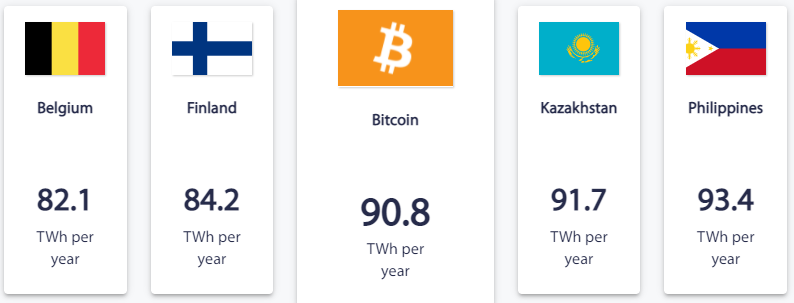
\includegraphics[width=\textwidth]{../../Figures/BTC_energy_consumption.png}
     \end{center}

\url{https://cbeci.org/}

\end{frame}


% \begin{frame}
% \bibliography{../../blockastics}
% \bibliographystyle{ieeetr}
% \end{frame}

\end{document}
